\subsubsection{Simulación de distintos modelos de batería}
Para que las simulaciones permitan obtener resultados fiables se buscó un modelo apropiado para la batería.
El primer modelo consta de una resistencia variable a partir de los datos obtenidos de los ensayos. 
Este componente representa la resistencia equivalente que presenta la batería,
que es responsable de la caída de tensión instantánea que se produce ante un escalón en la intensidad demandada.

El siguiente modelo propuesto añade un capacitor de muy alto valor en serie con la resistencia variable,
el cual representa la capacidad de almacenar carga de la batería.
El modelo actual es un modelo dinámico donde los valores de los componentes no son fijos,
sino que dependen de las condiciones de funcionamiento de la batería: estado de carga y funcionamiento en carga o descarga.

El circuito de la izquierda modela la resistencia interna de la batería y el comportamiento transitorio ante distintas cargas.
Por otro lado, el circuito de la derecha modela la capacidad de almacenamiento de energía de la batería y la carga almacenada durante los procesos de carga o descarga \cite{modelo_bateria_1}.

\begin{figure}
    \centering
    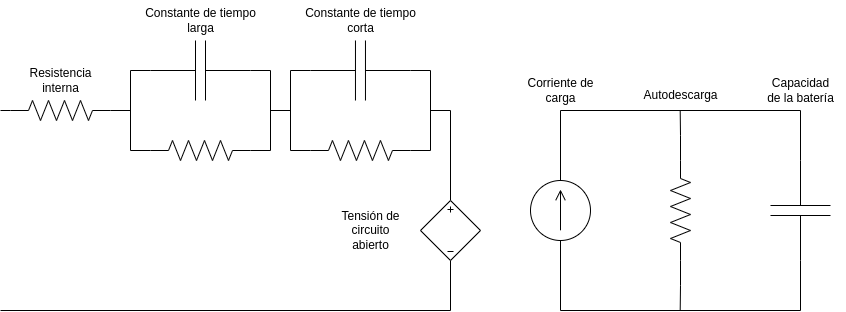
\includegraphics[width=\textwidth]{images/modelo_bateria.png}
    \caption{Modelo final de batería utilizado}
    \label{fig:bateria_3}
\end{figure}

Respecto al segundo modelo se agregan los siguientes componentes:
\begin{itemize}
    \item Los bloques compuestos por una resistencia y un capacitor en paralelo, que modelan la capacidad en los electrodos de las celdas y
    la resistencia no lineal entre electrodos y electrolito.
    En conjunto modelan las constantes de tiempo (corta y larga) de la respuesta transitoria de la tensión en la batería \cite{modelo_bateria_2}.
    \item La fuente de tensión controlada por tensión, que representa la dependencia no lineal entre el estado de carga ($SOC$)
    y la tensión de circuito abierto($V_{OC}$) dependiente del $SOC$.
    \item La fuente de corriente controlada por corriente, representa la corriente de carga que modifica el $SOC$.
\end{itemize}
La tensión que existe en el circuito secundario ($V_{SOC}$) se normaliza de forma que $V_{SOC}=1V$ equivale al $SOC (100\%)$.
La resistencia en paralelo modela la auto-descarga de la batería.